\documentclass{article}
\usepackage[utf8]{inputenc}
\usepackage{amsmath,color,amssymb,amsthm,mathrsfs,verbatim,tikz,graphicx}
\usepackage[margin=2.5cm]{geometry}
\usetikzlibrary{matrix,arrows,decorations.pathmorphing}
\theoremstyle{definition}
\newtheorem{defn}{Definition}
\newtheorem*{fact}{Fact}
\newtheorem{example}{Example}
\newtheorem*{ex}{Exercise}
\newtheorem*{soln}{Solution}
\newtheorem*{prob}{Problem}
\newtheorem*{lemma}{Lemma}

\theoremstyle{theorem}
\newtheorem{thm}{Theorem}

\newcommand{\R}{\mathbb{R}}
\newcommand{\A}{\mathbb{A}}
\newcommand{\Q}{\mathbb{Q}}
\newcommand{\Z}{\mathbb{Z}}
\newcommand{\X}{\mathbb{X}}
\newcommand{\Y}{\mathbb{Y}}
\newcommand{\N}{\mathbb{N}}
\newcommand{\M}{\mathbb{M}}
\newcommand{\C}{\mathbb{C}}
\newcommand{\E}{\mathbb{\emptyset}}
\newcommand{\F}{\mathbb{F}}
\newcommand{\Proj}{\mathbb{P}}
\newcommand{\HP}{\mathbb{H}}
\newcommand{\D}{\mathbb{D}}
\newcommand{\Pic}{\mbox{Pic}}
\newcommand{\Div}{\mbox{Div}}
\newcommand{\T}{\mathcal{T}}

\begin{document}

\title{Advanced Calculus HW 6 - Due October 13, 4pm}
\author{Luis Berlioz}
\maketitle



\begin{prob}[1]
Let $\mathbb{Z}$ be the two-point topological space with the discrete topology.  \\Prove that a topological space $\mathbb{M}$ is connected if and only if every continuous map from $\mathbb{M}$ to $\mathbb{Z}$ is constant.
\end{prob}
\begin{soln}
    We prove the counterpositive. First let us assume that there exists a continuous map $\M \to \Z$ such that it is not contant. This means that $f^{-1}(1)\neq$ and $f^{-1}(0) \neq 0$. These two sets are also open since they are the inverse image of open sets. And since $\Z = \{ 0, 1\}$ this means that $\M =  f^{-1}(0)\cup f^{-1}(1)  $. Therefore $\M$ is disconnected. 

    Next, assume that $\M$ is connected, then for any continuous function $f$, $f(\M)$ is also connected. Considering that the subsets of $\Z$ are $\E,\ \{0\},\ \{1\}, \{0,1\}$; we can conclude that the only connected subsets are $\{0\}$ and $\{1\}$ each of which makes $f$ a constant function.
\end{soln}
\vspace{1in}



\begin{prob}[2]
Let $\mathbb{X}$ be the polar curve in $\mathbb{R}^2$, given in polar co-ordinates by $\displaystyle{r = 1 - \frac{\pi}{\theta}}$, defined for real $\theta \ge \pi$.  \\Let $\mathbb{Y}$ be the topologist's sine curve in $\mathbb{R}^2$, given in Cartesian co-ordinates by  $\displaystyle{y = \sin\left(\frac{\pi}{x}\right)}$, defined for real $x\ge 0$.  
\begin{itemize}\item Sketch the curves $\mathbb{X}$ and $\mathbb{Y}$.
\item Prove that the spaces   $\mathbb{X}$ and $\mathbb{Y}$ are homeomorphic.
\item Prove that spaces $\overline{\mathbb{X}}$ and $\overline{\mathbb{Y}}$ are connected but not path connected.
\item Prove that the spaces $\overline{\mathbb{X}}$ and $\overline{\mathbb{Y}}$ are not homeomorphic.
\end{itemize}
\end{prob}
\begin{soln}
\begin{itemize}\item Sketch the curves $\mathbb{X}$ and $\mathbb{Y}$.
            \begin{figure}
  \centering
    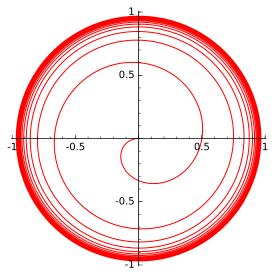
\includegraphics[width=0.5\textwidth]{figs/spiral.pdf}
  \caption{Polar graph of $r=1- \pi/\theta$}
\end{figure}
            \begin{figure}
  \centering
    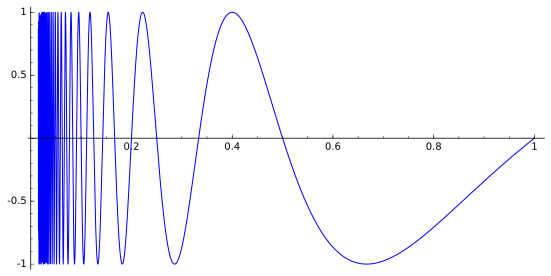
\includegraphics[width=0.5\textwidth]{figs/topol.pdf}
                \caption{Graph of $y = \sin(\pi/x)$}
\end{figure}
        \item The maps $\theta \mapsto (1-\pi/\theta, \theta)$ and $x \mapsto (x,\sin(\pi/x)$ where $\theta\geq \pi$ and $0<x\leq 1$ are both homeomorphisms. Since the sets (we proved this in the last homework) $[\pi,\infty)$ and $(0,1]$ are homeomorphic, we conclude that $\X$ and $\Y$ are homeomorphic.
\item Both $\X$ and $\Y$ are the image of connected spaces over continuous functions and therefore connected. In general, the closure of a connected set is connected because points in the closure cannot be disjoint from the original set. 

    First we show that $\Y$ is not path connected. Assuming it is, take a continuous function $\gamma\ :\ [0,1]\to \Y$ such that $\gamma(0) = (0,0)$ and $\gamma(1) = (1, 0)$

\item Prove that the spaces $\overline{\mathbb{X}}$ and $\overline{\mathbb{Y}}$ are not homeomorphic.
\end{itemize}

\end{soln}
\vspace{1in}


\begin{prob}[3]
The unit three-sphere $\mathbb{S}^3$, center the origin is the subset of $\mathbb{R}^4$, with Cartesian co-ordinates $(t, x, y, z) \in \mathbb{R}^4$ given by the equation $t^2 + x^2 + y^2 + z^2 = 1$.  \\Prove that $\mathbb{S}^3$ is connected.  Is $\mathbb{S}^3$ path connected?  Discuss.
\end{prob}
\begin{soln}

\end{soln}
\vspace{1in}




\begin{prob}[4]
For $r$ real, let $\mathbb{C}_r$ be the circle, center the point  $(r, 0) \in \mathbb{R}^2$ and radius $r$. \\ Define the Hawaiian earing, $\mathbb{H}$ and the one-sided Hawaiian earing, $\mathbb{H}_+$ by the formulas:
\[ \mathbb{H} =   \bigcup_{n \in (\mathbb{Z} - \{0\})} \mathbb{C}_{\frac{1}{n}}, \hspace{10pt} \mathbb{H}_+ =   \bigcup_{n \in \mathbb{N}} \mathbb{C}_{\frac{1}{n}}. \] 
Sketch $\mathbb{H}$ and $\mathbb{H}_+$.\\
Are these earings connected, or path connected? Explain. \\
Are $\mathbb{H}_+$ and $\mathbb{H}$ homeomorphic? Explain.\\
Also put $\mathbb{J} =  \bigcup_{n \in \mathbb{N}} \mathbb{C}_{n}$.\\
Sketch the set $\mathbb{J}$.\\
Is $\mathbb{J}$ homeomorphic to $\mathbb{H}$? Explain.\\
Also put $\mathbb{K} =  \bigcup_{r \in (\mathbb{R} - \{0\})} \mathbb{C}_{r}$.\\
Is the set $\mathbb{K}$ homeomorphic to $\mathbb{H}$? Explain.


\end{prob}
\begin{soln}

\end{soln}
\vspace{1in}


\begin{prob}[5]
Let $\mathbb{M}$ be the space of all continuous maps $f:[0, 1] \rightarrow \mathbb{R}$, equipped with the distance formula $d(f,g ) =  \sup\{ |f(x) - g(x)|:  x \in [0, 1]\}$.  \\Prove that $d$ gives the space $\mathbb{M}$ a metric.   \\For $n$ a positive integer, let $f_n(x) = x^n$, defined for any $x\in [0, 1]$. \\ Prove that the sequence $\mathbb{F} = \{f_n: n \in \mathbb{N}\}$ has no convergent subsequence. \\ Is $\mathbb{F}$ a Cauchy sequence? Explain. 
\end{prob}
\begin{soln}

\end{soln}
\vspace{1in}


\begin{prob}[6]
Prove that the closed real interval $[0, 1]$ cannot be written as a countably infinite disjoint union of intervals, each open in $[0, 1]$. 
\end{prob}
\begin{soln}

\end{soln}
\vspace{1in}



\end{document}








